% ══════════════════════════════════════════════════════════════════════
% CHAPTER 3: SYSTEM ARCHITECTURE
% ══════════════════════════════════════════════════════════════════════

\chapter{System Architecture}
\label{ch:architecture}

This chapter describes the system architecture of Seismic Viewer, detailing its structural decomposition, communication mechanisms, and execution model. The design balances two competing demands: the computational throughput required for data processing and the responsiveness expected of an interactive desktop application.

\section{Architectural Overview}
\label{sec:arch-overview}

\bluerevised{Seismic Viewer uses a client-server desktop architecture that combines a Python processing backend with an embedded Chromium frontend. The two layers communicate through three dedicated channels: a native bridge, HTTP REST endpoints, and WebSockets.}

\begin{figure}[htbp]
\centering
\begin{tikzpicture}[
    scale=0.74, transform shape,
    box_backend/.style={rectangle, draw=NavyBlue!80, fill=NavyBlue!10, rounded corners=4pt, minimum width=4.2cm, minimum height=1.35cm, align=center, font=\small},
    box_frontend/.style={rectangle, draw=OliveGreen!80, fill=OliveGreen!10, rounded corners=4pt, minimum width=4.2cm, minimum height=1.35cm, align=center, font=\small},
    container_backend/.style={rectangle, draw=NavyBlue!40, dashed, rounded corners=6pt, inner sep=16pt, fill=NavyBlue!3},
    container_frontend/.style={rectangle, draw=OliveGreen!40, dashed, rounded corners=6pt, inner sep=16pt, fill=OliveGreen!3},
    title_backend/.style={font=\bfseries\normalsize, text=NavyBlue!90},
    title_frontend/.style={font=\bfseries\normalsize, text=OliveGreen!90},
    proto_blue/.style={font=\footnotesize, fill=white, inner sep=3.5pt, draw=NavyBlue!40, text=NavyBlue!90, rounded corners=3pt},
    proto_green/.style={font=\footnotesize, fill=white, inner sep=3.5pt, draw=OliveGreen!40, text=OliveGreen!90, rounded corners=3pt},
    proto_red/.style={font=\footnotesize, fill=white, inner sep=3.5pt, draw=BrickRed!40, text=BrickRed!90, rounded corners=3pt}
]
    % Backend Nodes (All Blue = Python Backend Process at x = 0)
    \node[box_backend] (fastapi) at (0, 0) {\textbf{FastAPI Server}\\[-1pt]\footnotesize (REST \& WebSockets)};
    \node[box_backend] (bridge_py) at (0, -3.6) {\textbf{Bridge API}\\[-1pt]\footnotesize (\texttt{pywebview.js\_api})};
    \node[box_backend] (engine) at (0, -7.2) {\textbf{Analytical Engine}\\[-1pt]\footnotesize (NumPy, SciPy, scikit-learn)};
    
    % Frontend Nodes (All Green = Chromium Frontend Process at x = 10.5)
    \node[box_frontend] (web_client) at (10.5, 0) {\textbf{Network Layer}\\[-1pt]\footnotesize (Fetch \& WebSocket API)};
    \node[box_frontend] (ui_ctrl) at (10.5, -3.6) {\textbf{UI Controllers}\\[-1pt]\footnotesize (\texttt{window.pywebview.api})};
    \node[box_frontend] (plotly) at (10.5, -7.2) {\textbf{WebGL Visualisation}\\[-1pt]\footnotesize (Plotly.js 2D/3D/4D)};

    % Intra-process connections (Backend: Blue)
    \draw[{Stealth[length=2.5mm]}-{Stealth[length=2.5mm]}, thick, draw=NavyBlue!75] (fastapi.south) -- (bridge_py.north);
    \draw[{Stealth[length=2.5mm]}-{Stealth[length=2.5mm]}, thick, draw=NavyBlue!75] (bridge_py.south) -- (engine.north);

    % Intra-process connections (Frontend: Green)
    \draw[{Stealth[length=2.5mm]}-{Stealth[length=2.5mm]}, thick, draw=OliveGreen!75] (web_client.south) -- (ui_ctrl.north);
    \draw[{Stealth[length=2.5mm]}-{Stealth[length=2.5mm]}, thick, draw=OliveGreen!75] (ui_ctrl.south) -- (plotly.north);

    % Containers (Backgrounds matching Process colors)
    \begin{scope}[on background layer]
        \node[container_backend, fit=(fastapi) (engine), label={[title_backend]above:Python Backend Process}] (bg_backend) {};
        \node[container_frontend, fit=(web_client) (plotly), label={[title_frontend]above:Chromium Frontend Process}] (bg_frontend) {};
    \end{scope}

    % Inter-process communication channels (Horizontal lines with protocol-matched colors)
    % 1. HTTP REST API (Blue = Data Provider)
    \draw[-{Stealth[length=3.0mm]}, very thick, draw=NavyBlue] 
        ([yshift=5mm]fastapi.east) -- node[proto_blue, above=4pt] {HTTP REST (Float32 Binary / JSON)} ([yshift=5mm]web_client.west);

    % 2. WebSockets (Green = Live Client Duplex Stream)
    \draw[{Stealth[length=3.0mm]}-{Stealth[length=3.0mm]}, very thick, draw=OliveGreen] 
        ([yshift=-5mm]fastapi.east) -- node[proto_green, below=4pt] {WebSocket (4D Streams / Progress)} ([yshift=-5mm]web_client.west);

    % 3. Native Bridge RPC (Red = Native Inter-Process RPC Bridge)
    \draw[{Stealth[length=3.0mm]}-{Stealth[length=3.0mm]}, very thick, draw=BrickRed] 
        (bridge_py.east) -- node[proto_red] {JS-Python RPC Bridge} (ui_ctrl.west);

\end{tikzpicture}
\caption{Client-server architecture of Seismic Viewer with dedicated communication channels.}
\label{fig:arch-overview}
\end{figure}

\bluerevised{The architecture divides tasks across three dedicated communication channels, balancing responsiveness and data transfer speed:
\begin{enumerate}
    \item \textbf{Native Bridge}: Connects the user interface with the Python runtime for desktop actions. When the window opens, pywebview exposes methods of the Python \texttt{Api} class to JavaScript via \texttt{window.pywebview.api}. Actions such as selecting files or opening dialogs call these methods directly without network delay.
    \item \textbf{HTTP REST Endpoints}: Handles data transfer between backend and frontend. Rather than embedding large datasets into HTML pages, the frontend requests catalogs asynchronously. Numerical coordinates are streamed as Float32 binary buffers via \texttt{/api/data/\{id\}/bin}, while catalog metadata and views are served with standard compression.
    \item \textbf{WebSockets}: Manages live updates and streaming during long calculations. When running temporal animations or clustering routines, the backend streams progress notifications and frame updates directly to the client over an open connection, updating the interface without page reloads.
\end{enumerate}
\Cref{tab:rest-api} lists the REST endpoints and WebSocket message types supported by the system.}

\begin{table}[htbp]
\centering
\caption{REST API endpoints and WebSocket message protocol.}
\label{tab:rest-api}
\footnotesize
\renewcommand{\arraystretch}{1.1}
\begin{tabularx}{\textwidth}{@{}l l >{\raggedright\arraybackslash}X@{}}
\toprule
\textbf{Protocol / Endpoint} & \textbf{Direction / Path} & \textbf{Description / Message Types} \\
\midrule
REST (\texttt{GET}) & \texttt{/api/data/\{session\_id\}} & Retrieve session data as GZip-compressed JSON \\
REST (\texttt{GET}) & \texttt{/api/data/\{session\_id\}/bin} & Retrieve numerical data as Float32 binary buffer \\
REST (\texttt{GET}) & \texttt{/viz/\{viz\_id\}} & Serve pre-rendered HTML visualisation page \\
\midrule
WebSocket & Client $\to$ Server & \texttt{ping}, \texttt{get\_cluster\_update}, \texttt{get\_structural\_planes}, \texttt{get\_animated\_clustering} \\
WebSocket & Server $\to$ Client & \texttt{pong}, \texttt{rpc\_response}, \texttt{progress} (broadcast messages) \\
\bottomrule
\end{tabularx}
\end{table}

\section{Backend Architecture}
\label{sec:backend}

\subsection{Application Entry Point \& Bridge Engine}
\label{sec:bridge}

Once the application is running, the \texttt{Api} module acts as the central coordinator. Whenever the user interacts with the interface, such as selecting a file (\texttt{select\allowbreak\_csv()}), loading a 3D view (\texttt{load\allowbreak\_view()}), or exporting results (\texttt{export\allowbreak\_clusters\allowbreak\_csv()}), the frontend sends a request directly to this coordinator.

\bluerevised{These requests include spatial analysis calculations on seismic events. To prevent blocking the graphical interface during execution, operations run on background workers using threads or process pools. The application sends progress updates from worker threads to the WebSocket event loop without conflicts.}

Since the calculations occur in the background, the application requires a mechanism to inform the user about the ongoing progress. The coordinator handles this requirement by continuously transmitting real-time updates back to the interface. This ensures the user is constantly provided with a responsive progress bar or status message, resulting in a fluid and stable user experience. These updates are broadcast through the WebSocket protocol.

\subsection{Session Store \& FastAPI Middleware}
\label{sec:session-store}

The system architecture requires a dedicated memory management layer to preserve state between user interactions and to serve data efficiently to the graphical frontend. This functionality is centralized within an internal configuration module (\texttt{core/config.py}), which orchestrates two separate in-memory caches: \texttt{\_data\_store} and \texttt{\_html\_store}.

The \texttt{\_data\_store} structure retains the raw numerical arrays and metadata associated with each active analytical session. To guarantee that the application maintains a stable memory profile even during extensive analytical workflows, this cache is strictly limited to 30 concurrent sessions. In parallel, the \texttt{\_html\_store} caches up to 15 pre-rendered graphical views, allowing the frontend to load complex tridimensional scenes instantaneously. Both structures implement a First-In, First-Out (FIFO) eviction policy. \bluerevised{To ensure safety during simultaneous operations, updates to these stores are synchronized, keeping application memory use low during long sessions.}

Positioned between this caching layer and the client interface, the FastAPI server deploys specific middleware to optimize network throughput. An important optimization is the automatic application of GZip compression for any outgoing data payload larger than 500 bytes. Compressing the data prior to transmission accelerates the rendering process, particularly when transferring datasets containing tens of thousands of seismic events.

\section{Frontend Architecture}
\label{sec:frontend}

\subsection{Single-Page Application \& UI/UX Design}
\label{sec:spa}

As illustrated in \Cref{fig:gui-hub}, the primary workflow begins at the landing screen (\subref{fig:start-page}). Here, the system exposes multiple data ingestion pathways, allowing researchers to import local csv files, query the INGV remote web services directly, or restore a previously interrupted session through local historical records.

\bluerevised{Once the imported dataset is validated, the software opens the visualization hub (\subref{fig:viz-hub}). This view provides menus to switch between the available display modes and clustering algorithms. In addition, it includes toggles to display extra data layers on the 3D map, such as seismic tomography, ground uplift, and monitoring stations.}

\bluerevised{The 3D graphics pipeline delegates rendering to WebGL through Plotly.js. To preserve context during updates, the system retains the view angle and zoom level selected by the user. This prevents the camera from resetting when new data arrives, maintaining smooth interaction (\Cref{sec:challenge-camera}).}

\begin{figure}[H]
\centering
\begin{subfigure}{0.48\textwidth}
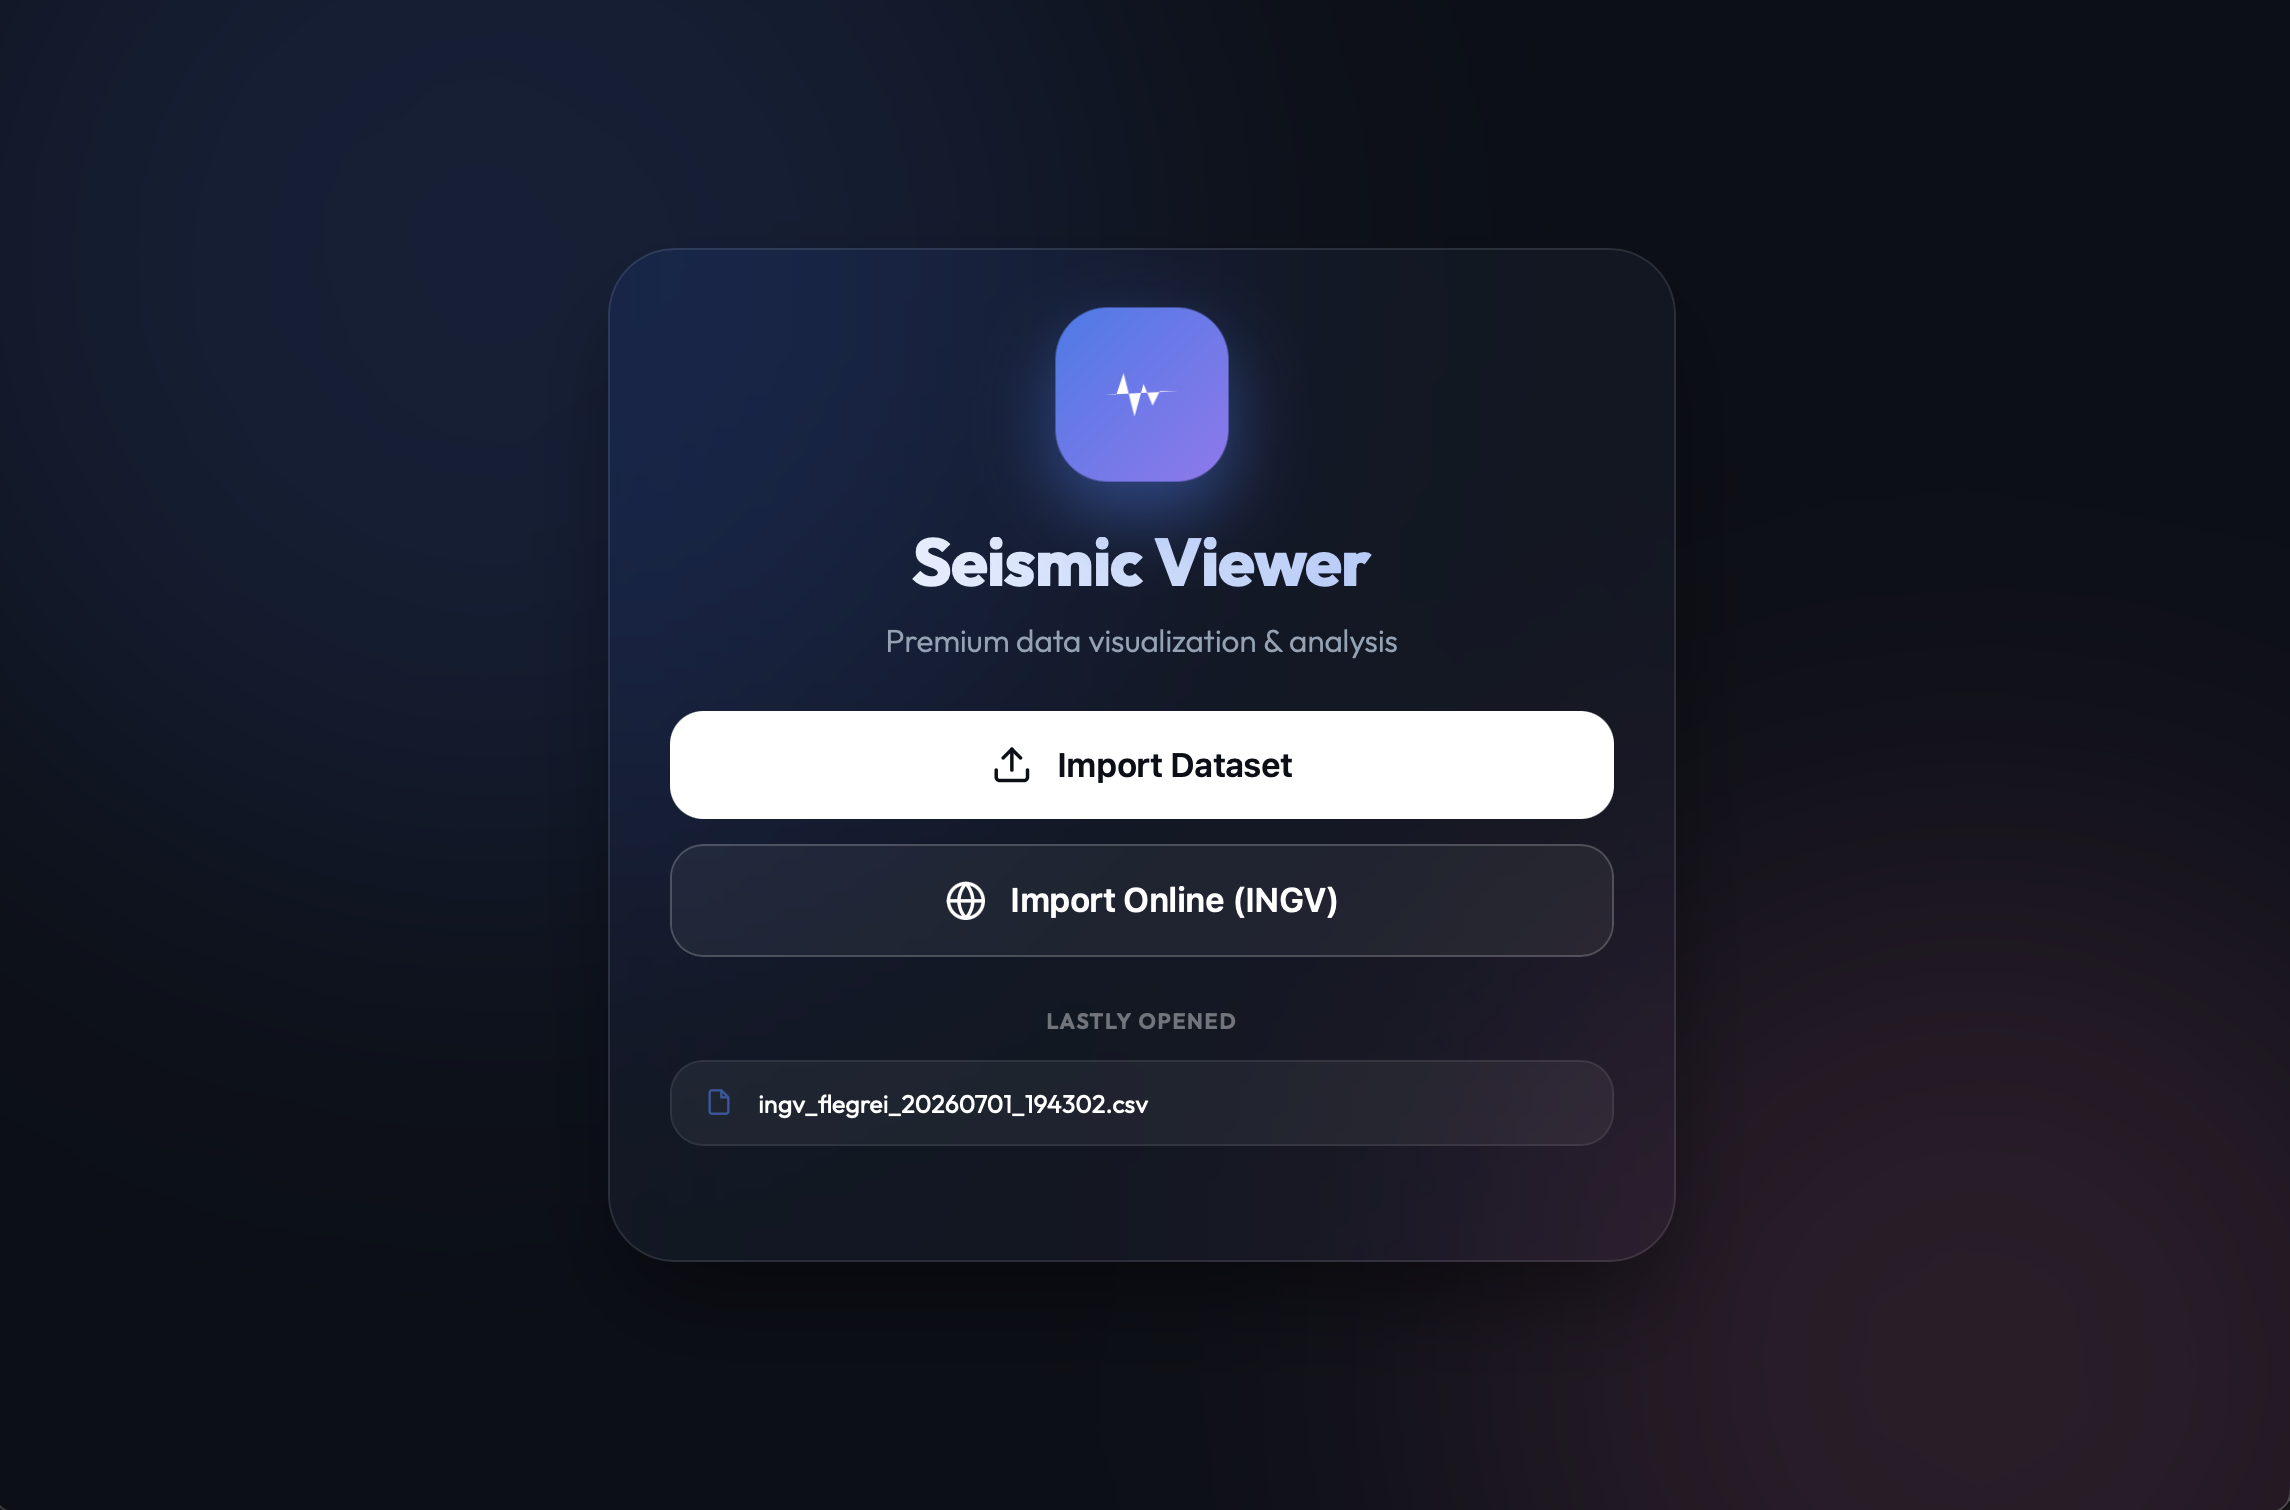
\includegraphics[width=\textwidth]{images/start_page.png}
\caption{File Picker view.}
\label{fig:start-page}
\end{subfigure}\hfill
\begin{subfigure}{0.48\textwidth}
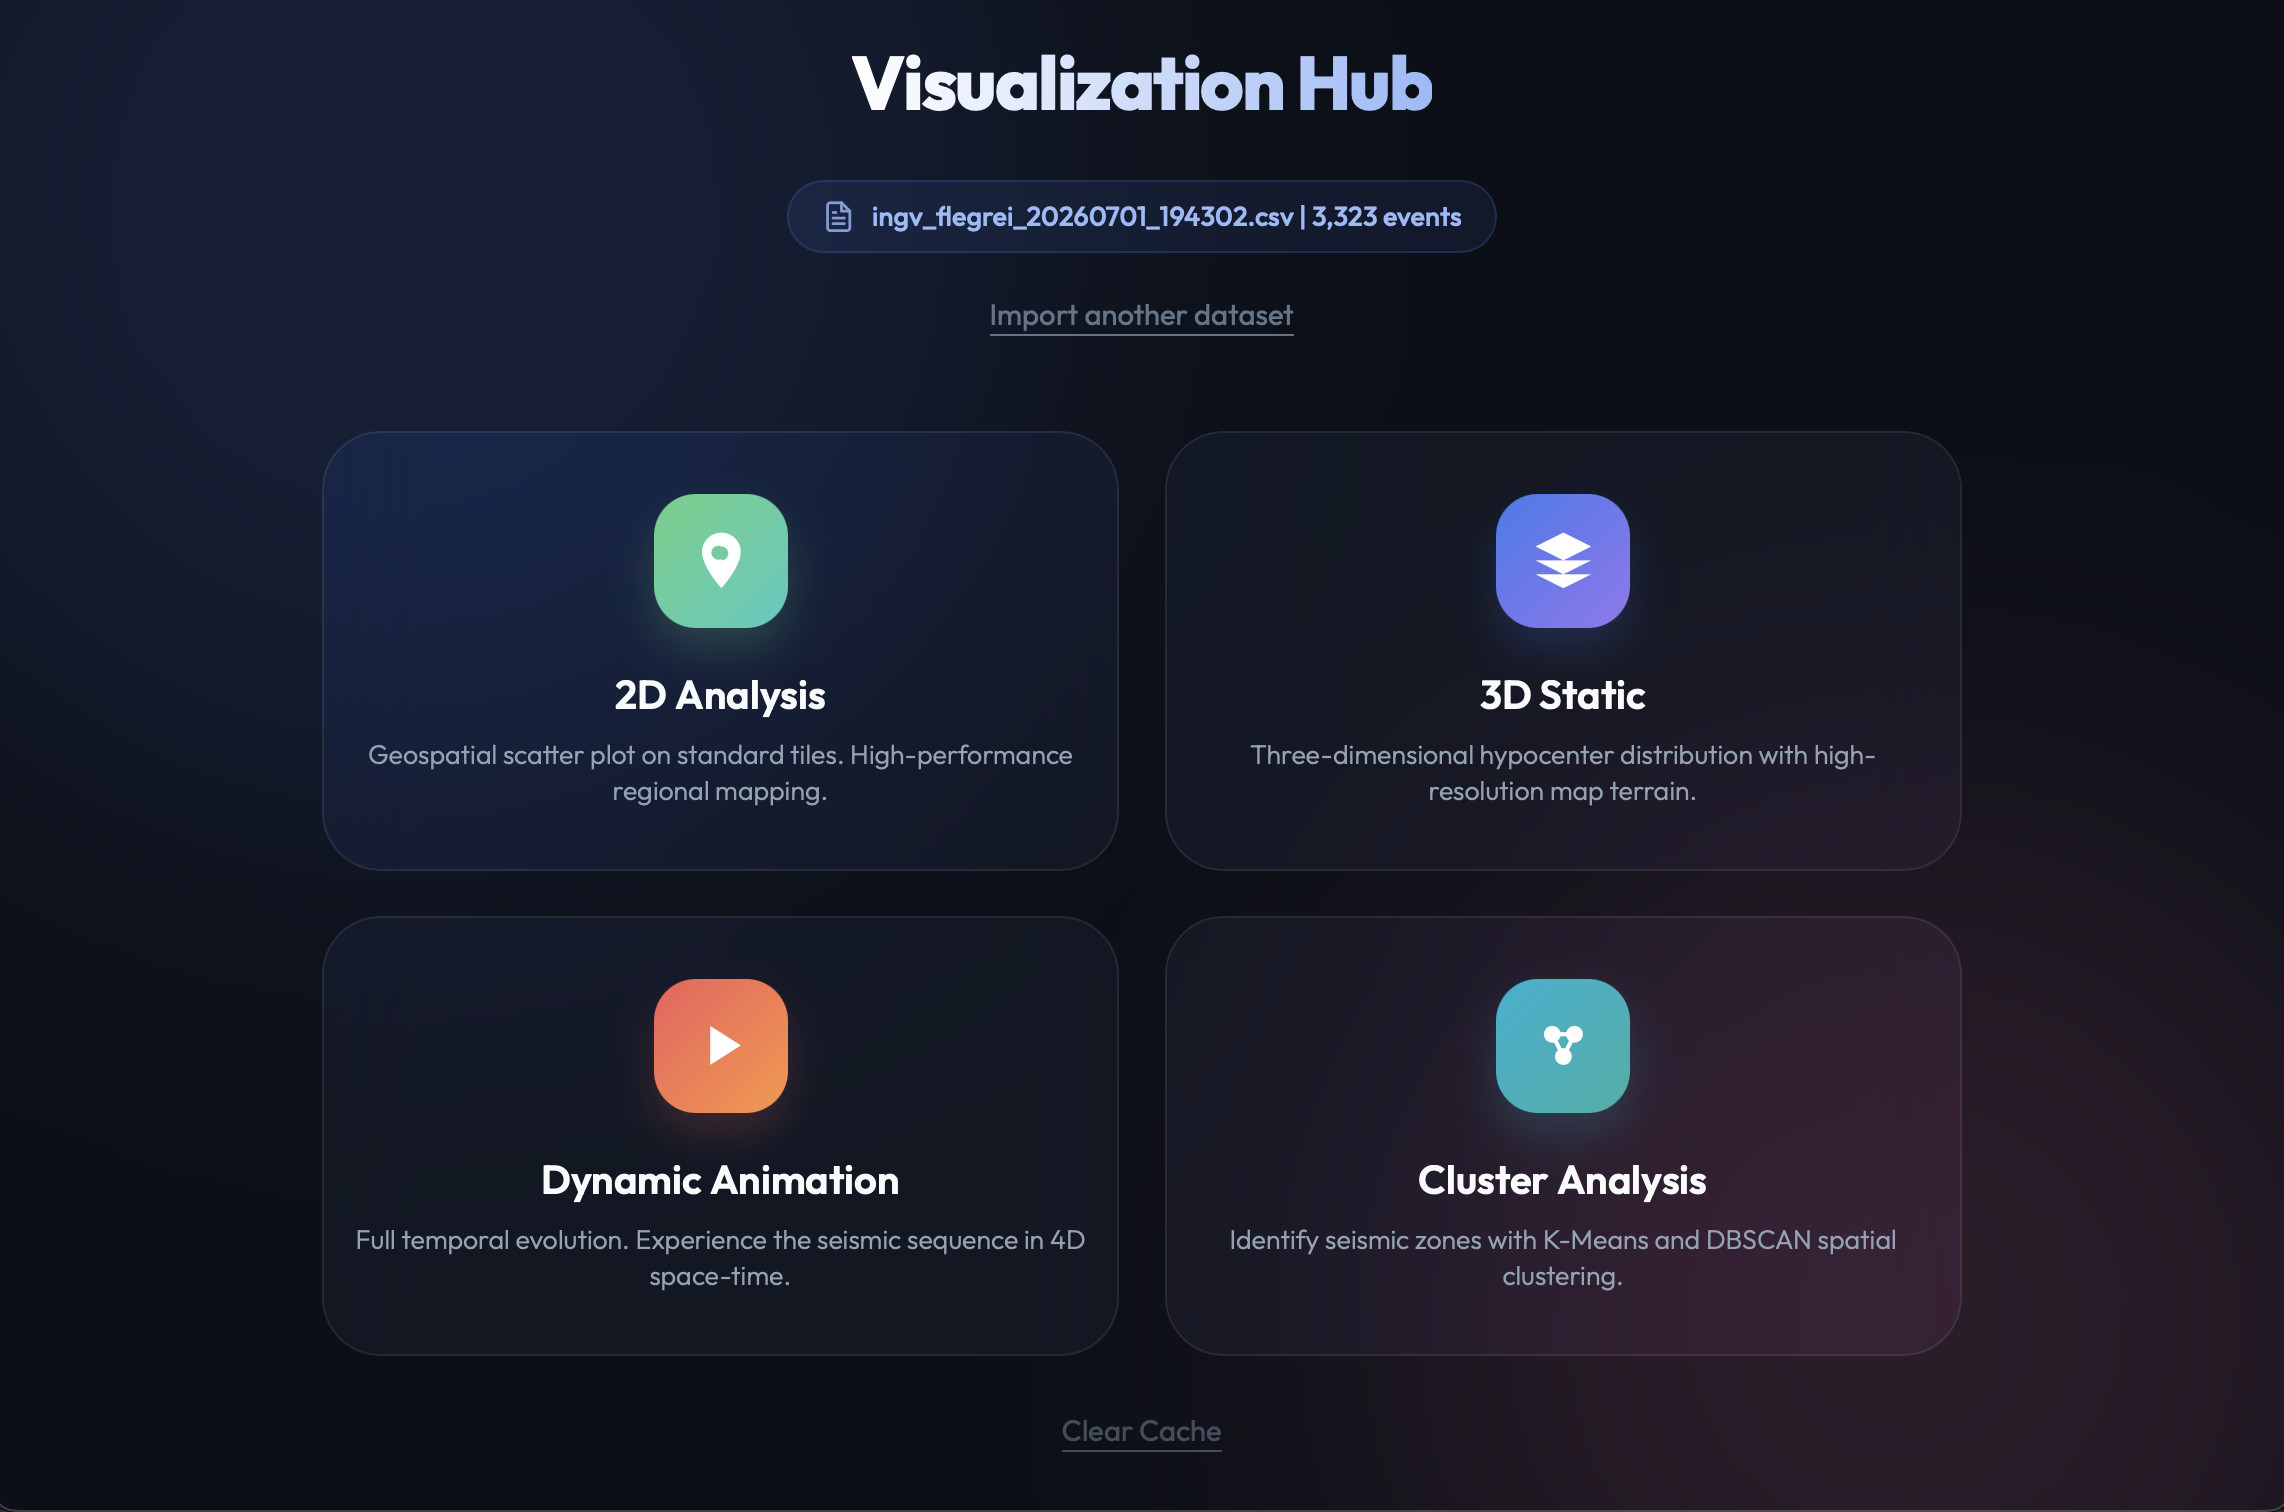
\includegraphics[width=\textwidth]{images/visualization_hub.png}
\caption{Visualisation Hub with mode selection.}
\label{fig:viz-hub}
\end{subfigure}
\caption{The Seismic Viewer single-page application structure, showing initial data loading (\subref{fig:start-page}) and the multi-mode analytical selection hub (\subref{fig:viz-hub}).}
\label{fig:gui-hub}
\end{figure}

\section{Data Flow Pipeline and Protocols}
\label{sec:dataflow}
\label{sec:protocols}

\bluerevised{To manage data processing and rendering, Seismic Viewer divides operations between backend services and the frontend client. On the backend, the system handles data loading, validation, and mathematical calculations. As shown in \Cref{fig:dataflow}, the pipeline begins by importing CSV data or querying the INGV API. This data is cleaned and loaded. Visual pre-computations prepare coordinate structures before the engine executes the selected algorithm. Finally, results are stored in the internal caches and rendered in HTML.}

\begin{figure}[H]
\centering
\begin{tikzpicture}[node distance=1.4cm, auto, scale=0.82, transform shape]
    \node (input) [io] {CSV / INGV API};
    \node (loader) [process, below of=input] {Loader \& Sanitisation};
    \node (precomp) [process, below of=loader] {Visual Pre-computation};
    \node (decision) [decision, below of=precomp, yshift=-0.2cm] {View Style?};
    \node (engine) [process, below of=decision, yshift=-0.4cm] {Engine (Viz/Analysis)};
    \node (template) [process, below of=engine] {HTML Template Assembly};
    \node (store) [io, below of=template] {Session Store + HTML Store};
    \node (render) [startstop, below of=store] {WebGL Rendering};

    \draw [arrow] (input) -- (loader);
    \draw [arrow] (loader) -- (precomp);
    \draw [arrow] (precomp) -- (decision);
    \draw [arrow] (decision) -- node[left, font=\scriptsize] {0/1/2/3/4} (engine);
    \draw [arrow] (engine) -- (template);
    \draw [arrow] (template) -- (store);
    \draw [arrow] (store) -- (render);
    \begin{pgfinterruptboundingbox}
    \draw [dashedarrow] (store.east) -- ++(2.4,0) node[right, font=\scriptsize, text width=3.2cm] {Binary Float32 buffer via \texttt{/api/data/\{id\}/bin}};
    \end{pgfinterruptboundingbox}
\end{tikzpicture}
\caption{Linear data pipeline from input parsing to WebGL drawing.}
\label{fig:dataflow}
\end{figure}

Once the backend processing is complete, the frontend retrieves the data through the defined REST API and WebSocket endpoints (\Cref{tab:rest-api}). The frontend dynamically renders the 3D scene using WebGL via the Plotly.js library. Continuous status updates, real-time recalculations, and filtering commands are exchanged over the WebSocket channel, ensuring the interface remains fully interactive without needing page reloads.

\begin{figure}[htbp]
\centering
\begin{tikzpicture}[scale=0.82, transform shape,
    lifeline/.style={draw=black!40, dashed, thick},
    msg/.style={-Stealth, thick},
    actor/.style={rectangle, draw=NavyBlue!80, fill=NavyBlue!10, rounded corners=3pt, minimum width=2.4cm, minimum height=0.8cm, font=\footnotesize\bfseries, align=center}
]
    \node[actor] (ui) at (0, 0) {Chromium UI};
    \node[actor] (bridge) at (3.6, 0) {Native Bridge};
    \node[actor] (worker) at (7.2, 0) {Worker Thread};
    \node[actor] (fastapi) at (10.8, 0) {FastAPI Server};

    \draw[lifeline] (ui) -- (0, -5.2);
    \draw[lifeline] (bridge) -- (3.6, -5.2);
    \draw[lifeline] (worker) -- (7.2, -5.2);
    \draw[lifeline] (fastapi) -- (10.8, -5.2);

    \draw[msg, draw=BrickRed] (0, -0.8) -- node[above, font=\scriptsize] {1. Action: \texttt{trigger\_cluster()}} (3.6, -0.8);
    \draw[msg, draw=NavyBlue] (3.6, -1.4) -- node[above, font=\scriptsize] {2. Spawn worker} (7.2, -1.4);
    \draw[msg, draw=OliveGreen] (7.2, -2.0) -- node[above, font=\scriptsize] {3. Progress (WebSocket)} (10.8, -2.0);
    \draw[msg, draw=OliveGreen] (10.8, -2.4) -- node[above, font=\scriptsize] {4. Broadcast progress} (0, -2.4);
    \draw[msg, draw=NavyBlue] (7.2, -3.2) -- node[above, font=\scriptsize] {5. Store results in cache} (10.8, -3.2);
    \draw[msg, draw=NavyBlue] (0, -3.8) -- node[above, font=\scriptsize] {6. HTTP GET \texttt{/bin}} (10.8, -3.8);
    \draw[msg, draw=NavyBlue] (10.8, -4.3) -- node[above, font=\scriptsize] {7. Float32 ArrayBuffer} (0, -4.3);
    \node[fill=OliveGreen!15, draw=OliveGreen!60, rounded corners=3pt,
          font=\scriptsize, inner sep=3pt, anchor=west]
          at (0.12, -4.8) {8. Direct WebGL Render};
\end{tikzpicture}
\caption{Sequence diagram of asynchronous execution and non-blocking streaming pipeline.}
\label{fig:seq-diagram}
\end{figure}

\subsection{Binary Data Transfer Protocol}
\label{sec:binary-protocol}

To eliminate JSON parsing overhead during large catalog transfers, the backend packs numerical coordinates into a contiguous Float32 buffer (\texttt{/api/data/\{id\}/bin}) structured as: header \texttt{[event\_count, cluster\_count]} followed sequentially by arrays for longitude, latitude, magnitude, depth, \texttt{dates\_num}, and cluster labels ($C$ floats).

\begin{table}[htbp]
\centering
\caption{Binary buffer layout (Float32).}
\label{tab:binary-layout}
\footnotesize
\renewcommand{\arraystretch}{1.1}
\begin{tabular}{@{}l l | l l@{}}
\toprule
\textbf{Offset} & \textbf{Content} & \textbf{Offset} & \textbf{Content} \\
\midrule
0 (2 floats) & Header: \texttt{[N, C]} & $2+3N$ ($N$ floats) & Depth array \\
2 ($N$ floats) & Longitude array & $2+4N$ ($N$ floats) & Dates\_num array \\
$2+N$ ($N$ floats) & Latitude array & $2+5N$ ($C$ floats) & Cluster labels (if present) \\
$2+2N$ ($N$ floats) & Magnitude array & & \\
\bottomrule
\end{tabular}
\end{table}

\bluerevised{On the frontend, decoding via JavaScript's \texttt{Float32Array} directly over an \texttt{ArrayBuffer} completes in a few milliseconds even for large datasets, reducing transfer volume by approximately 80\% and avoiding JSON parsing delays.}

\section{Threading and Concurrency Model}
\label{sec:threading}

\begin{figure}[htbp]
\centering
\begin{tikzpicture}[node distance=1.5cm and 4.2cm, scale=0.86, transform shape]
    \node[module, minimum width=3.6cm, fill=OliveGreen!15] (main) {Main Thread (pywebview)};
    \node[module, minimum width=3.6cm, fill=NavyBlue!15, right=4.2cm of main] (uvicorn) {Daemon Thread (Uvicorn)};
    \node[module, minimum width=3.6cm, fill=orange!15, below=1.4cm of main] (worker) {Worker Thread (Analysis)};
    \node[module, minimum width=3.6cm, fill=BrickRed!15, below=1.4cm of uvicorn] (asyncio) {asyncio Event Loop};

    \draw[arrow] (main) -- node[above, font=\scriptsize] {starts} (uvicorn);
    \draw[arrow] (main) -- node[left, font=\scriptsize] {spawns} (worker);
    \draw[arrow] (uvicorn) -- node[right, font=\scriptsize] {hosts} (asyncio);
    \draw[dashedarrow] (worker) -- node[above=2pt, font=\scriptsize\ttfamily] {run\_coroutine\_threadsafe} (asyncio);
\end{tikzpicture}
\caption{Concurrency hierarchy linking UI, server thread, and analysis worker threads.}
\label{fig:threading}
\end{figure}

The concurrency architecture separates responsibilities across the \textbf{Main Thread} (hosting pywebview and Chromium), the \textbf{Server Thread} (running the Uvicorn \cite{uvicorn} asyncio event loop), and on-demand \textbf{Worker Threads} handling view generation and clustering updates. For intensive multi-frame calculations (animated clustering and RANSAC+SVD plane tracking), the engine escalates to a \texttt{ProcessPoolExecutor} with up to 8 worker processes utilising shared memory initialisers to avoid array serialisation. \bluerevised{This concurrency model prevents lock contention during numerical loops, ensuring the interface remains smooth and responsive during intensive calculations.}
